% ========== Template by IC\M/T Institute of Creative\Media/Technologies =============
% ==========  M. Wagner and K. Blumenstein, 2021 ============= 
% ==========  Based on the LaTeX Thesis Template for the University of Applied Sciences St.Pölten by P. Lechner https://github.com/hrtlacek/ThesisTemplate-FH-StP        ============= 

%----------------------------------------------------------------
% TODO List


%----------------------------------------------------------------

% ============= Settings for the Work =============

%***************************************************************************************

% Place your data here!!!

\def\workTitle{Field Theories \& \\ Canonical Quantization}
\def\subTitle{~}
\def\specialization{<Name of Masterclass>}
\def\studentFirstName{Mukund V, Pugazharasu A D, and Rishi Kumar}
%\def\studentLastName{A D}
\def\studentId{18-UPH-311, 18-UPH-313, 18-UPH-347}
\def\advisorPreTitle{Prof.}
\def\advisoFirstName{T. R.}
\def\advisorLastName{Govindarajan}
\def\advisorPosTitle{Adjunct Factuly, IMSc, Chennai}
\def\assessorPreTitle{Dr.}
\def\assessorFirstName{A. Stanley}
\def\assessorLastName{Raj}
\def\assessorPosTitle{Assistant Professor, Loyola Colelge, Chennai}
\def\place{Loyola College, Chennai}
\def\dateDay{25}
\def\dateMonth{04}
\def\dateYear{2021}

%***************************************************************************************

\newif\ifUseOneSide                         % <== DONT TOUCH THIS!!!
\newif\ifUseGermanVersion				    % <== DONT TOUCH THIS!!!
\newif\ifUseMasterInteractiveTechnologies 	% <== CAN'T TOUCH THIS!!! (da da dada)
\newif\ifUseMasterDigitalDesign	            % <== DONT TOUCH THIS!!!
\newif\ifUseMasterDigitalMediaProduction	% <== DONT TOUCH THIS!!!
\newif\ifUseMasterDigitalHealthCare			% <== DONT TOUCH THIS!!!
\newif\ifUseBachelorMediaTechnologiesOne    % <== DONT TOUCH THIS!!!
\newif\ifUseBachelorMediaTechnologiesTwo    % <== DONT TOUCH THIS!!!
\newif\ifUseBachelorSmartEngineeringOne     % <== DONT TOUCH THIS!!!
\newif\ifUseBachelorSmartEngineeringTwo     % <== DONT TOUCH THIS!!!
\newif\ifUseBachelorCreativeComputingOne    % <== DONT TOUCH THIS!!!
\newif\ifUseBachelorCreativeComputingTwo    % <== DONT TOUCH THIS!!!

%To switch between one or two side layout
\UseOneSidetrue                             % Using the one side layout
%\UseOneSidefalse                            % Using the two side layout
% *** ATTENTION: When using double page layout, you need to print the Title Page as a single Page!!! ***

%***************************************************************************************

% To switch the version please use the comment "%" option :-). After a language change, you have to rebuild the whole project (in Overleaf --> recompile from scratch) 
%\UseGermanVersiontrue					    % German version
\UseGermanVersionfalse					    % English version

%***************************************************************************************

% To switch between the study programs use the comment option :-) 
% !!!ATTENTION: Only one has to be activated!!!
%\UseBachelorMediaTechnologiesOnetrue		% Bachelor #1 Media Technology
%\UseBachelorMediaTechnologiesTwotrue		% Bachelor #2 Media Technology
%\UseBachelorSmartEngineeringOnetrue		% Bachelor #1 Smart Engineering
%\UseBachelorSmartEngineeringTwotrue		% Bachelor #2 Smart Engineering
%\UseBachelorCreativeComputingOnetrue		% Bachelor #1 Creative Computing
%\UseBachelorCreativeComputingTwotrue		% Bachelor #2 Creative Computing
\UseMasterInteractiveTechnologiestrue		% Master Interactive Technologies
%\UseMasterDigitalDesigntrue		        % Master Digital Design
%\UseMasterDigitalMediaProductiontrue		% Master Digital Media Production
%\UseMasterDigitalHealthCaretrue			% Master Digital Health Care

%***************************************************************************************

%Dokumentklasse without end dot ;-)
%\documentclass[a4paper,twoside,11pt, numbers=noenddot]{scrreprt}
\ifUseOneSide
    \documentclass[a4paper,oneside,11pt, numbers=noenddot]{scrreprt}%{book}{report}
\else
    \documentclass[a4paper,twoside,11pt, numbers=noenddot]{scrreprt}%{book}{report}
\fi

\usepackage[left= 3.5cm,right = 3cm, bottom = 3.5 cm, top = 3 cm]{geometry}
\usepackage[onehalfspacing]{setspace}
\usepackage{physics}
\usepackage{biblatex}
\addbibresource{Bibliography.bib}
\usepackage{tcolorbox}
\tcbuselibrary{skins}
\usepackage{lipsum}
\usepackage{amsmath}
% Standard Packages
\usepackage[utf8]{inputenc}

% ============= Packages =============

% Document information
\usepackage[
	pdftitle={\workTitle},
	pdfsubject={},
	pdfauthor={\studentFirstName \studentLastName},
	pdfkeywords={}
	pdftex=true, 
	colorlinks=true,
 	breaklinks=true,
	citecolor=black,
	linkcolor=black,	
	menucolor=black,	
	urlcolor=black
]{hyperref}

\hypersetup{
    %bookmarks=true,         % show bookmarks bar?
    unicode=false,          % non-Latin characters in Acrobat’s bookmarks
    pdftoolbar=true,        % show Acrobat’s toolbar?
    pdfmenubar=true,        % show Acrobat’s menu?
    pdffitwindow=false,     % window fit to page when opened
    pdfstartview={FitH},    % fits the width of the page to the window
    pdftitle={My title},    % title
    pdfauthor={Author},     % author
    pdfsubject={Subject},   % subject of the document
    pdfcreator={Creator},   % creator of the document
    pdfproducer={Producer}, % producer of the document
    pdfkeywords={keyword1} {key2} {key3}, % list of keywords
    pdfnewwindow=true,      % links in new window
    colorlinks=false,       % false: boxed links; true: colored links
    linkcolor=black,          % color of internal links (change box color with linkbordercolor)
    citecolor=black,        % color of links to bibliography
    filecolor=black,      % color of file links
    urlcolor=black           % color of external links
}

\usepackage{csquotes}

\usepackage[T1]{fontenc}
\usepackage{graphicx, subfigure}
\usepackage{fancyhdr}
\usepackage{lmodern}
\usepackage{color}
\usepackage{transparent}

\usepackage[backend=biber, style=apa, citestyle=authoryear, sorting=nyt]{biblatex}

% Switch the language
\ifUseGermanVersion
    \DeclareLanguageMapping{ngerman}{ngerman-apa}
\else
    \DeclareLanguageMapping{english}{english-apa}
\fi

\addbibresource{biblatex.bib}

% Additional letters from the American Mathematical Society
\usepackage{amsfonts}
\usepackage{mathtools}

\usepackage[export]{adjustbox}

% Block Diagram Drawing Package
% ---tikz
\usepackage{tikz}
\usetikzlibrary{positioning}
\usepackage{pgfplots}
\pgfplotsset{compat=1.10}
\usepackage{textcomp}

%Package for using the [H] option on graphics to force them into place
\usepackage{float}

%iPython packages:
%\usepackage{graphicx} % Used to insert images
\usepackage{adjustbox} % Used to constrain images to a maximum size 
\usepackage{color} % Allow colors to be defined
\usepackage{enumerate} % Needed for markdown enumerations to work
\usepackage{geometry} % Used to adjust the document margins
\usepackage{amsmath} % Equations
\usepackage{amssymb} % Equations
%\usepackage[mathletters]{ucs} % Extended unicode (utf-8) support
% \usepackage[utf8x]{inputenc} % Allow utf-8 characters in the tex document
\usepackage{fancyvrb} % verbatim replacement that allows latex
\usepackage{grffile} % extends the file name processing of package graphics 
                         % to support a larger range 
    % The hyperref package gives us a pdf with properly built
    % internal navigation ('pdf bookmarks' for the table of contents,
    % internal cross-reference links, web links for URLs, etc.)
\usepackage{hyperref}
\usepackage{longtable} % longtable support required by pandoc >1.10

% embedding of audio/video files etc.
% \usepackage{attachfile}
% \usepackage{movie15}
% \usepackage{media9}
% \usepackage{menukeys}

\usepackage[labelfont=it, labelsep=period, format=plain,justification=raggedright, singlelinecheck=false]{caption}
\captionsetup[figure]{justification=centering}
\definecolor{light-gray}{gray}{0.85}

% Switch between German and English based on the Settingx.tex. file
\usepackage{ifthen}

% =============== Block Diagram Drawing Config
\usetikzlibrary{shapes,arrows}

% Definition of blocks:
\tikzset{%
  block/.style    = {draw, thick, rectangle, minimum height = 3em,
    minimum width = 3em},
  sum/.style      = {draw, circle, node distance = 2cm}, % Adder
  input/.style    = {coordinate}, % Input
  output/.style   = {coordinate}, % Output
  mult/.style	  = {draw, isosceles triangle, minimum height=1cm, minimum width =1cm}
}
%mult/.style	  = {isosceles triangle, sharp corners, anchor=center, xshift=-4mm, minimum height=1.5cm, minimum width =0.05cm}
%isosceles triangle, fill=gray!25, minimum width=1.5cm

% Defining string as labels of certain blocks.
\newcommand{\suma}{\Large$+$}
\newcommand{\inte}{$\displaystyle \int$}
\newcommand{\derv}{\huge$\frac{d}{dt}$}
\newcommand{\conv}{\huge$\ast$}

% ============================================

% -- Settings für Code abbildungen
\usepackage{listings,lstautogobble}
\lstset{backgroundcolor=\color{light-gray},frame=single, framerule=0pt, showspaces=false, showtabs=false, numbers=left, numbersep=5pt, breaklines=false, autogobble=true, language=C++}

% Setze arial font
\usepackage[scaled]{helvet}
\renewcommand*{\familydefault}{\sfdefault}

% FH-green blue
\definecolor{FH}{rgb}{0.10, 0.57, 0.68}
% FH-green blue 2
\definecolor{FH2}{rgb}{0.0392, 0.666, 0.549}

% No indention afer a paragraph
\setlength{\parindent}{0cm}

% Paragraph
\setlength{\parskip}{0.3cm}

% ============= Header and Footer =============

\renewcommand{\chaptermark}[1]{\markboth{\thechapter~ #1}{}}

\ifUseOneSide
\fancypagestyle{icmt}{%
  \fancyhf{}% Clear header and footer
  \fancyhead[L]{\leftmark}
  \fancyfoot[R]{\thepage}% Custom footer
  \renewcommand{\headrulewidth}{0.4pt}% Line at the header visible
  \renewcommand{\footrulewidth}{0.0pt}% Line at the footer visible
}
% Redefine the plain page style
\fancypagestyle{plain}{%
  \fancyhf{}%
  \fancyfoot[R]{\thepage}%
  \renewcommand{\headrulewidth}{0.0pt}% Line at the header invisible
  \renewcommand{\footrulewidth}{0.0pt}% Line at the footer visible
}
\else
\fancypagestyle{icmt}{%
  \fancyhf{}% Clear header and footer
  \fancyhead[L]{\leftmark}
  \fancyfoot[RO,LE]{\thepage}% Custom footer
  \renewcommand{\headrulewidth}{0.4pt}% Line at the header visible
  \renewcommand{\footrulewidth}{0.0pt}% Line at the footer visible
}
% Redefine the plain page style
\fancypagestyle{plain}{%
  \fancyhf{}%
  \fancyfoot[RO,LE]{\thepage}%
  \renewcommand{\headrulewidth}{0.0pt}% Line at the header invisible
  \renewcommand{\footrulewidth}{0.0pt}% Line at the footer visible
  }
\fi

% ============= Package Settings & Others ============= 


% Special Spellings
\hyphenation{De-zi-mal-tren-nung St-rei-fen-licht-scan-nern}

% Roman itemization \RM{<Number>}
\newcommand{\RM}[1]{\MakeUppercase{\romannumeral #1}}


% ============= Dokumentbeginn =============

\begin{document}

% Select the right main page ;-)
\ifUseGermanVersion
	
% setup page dimensions for titlepage
\newgeometry{left=2.4cm,right=2.4cm,bottom=2.5cm,top=2cm}

% force baselineskip and parindent
%\newlength{\tmpbaselineskip}
%\setlength{\tmpbaselineskip}{\baselineskip}
%\setlength{\baselineskip}{13.6pt}
%\newlength{\tmpparindent}
%\setlength{\tmpparindent}{\parindent}
%\setlength{\parindent}{17pt}

% first titlepage
\pagestyle{empty}

\begin{figure}[H]
\vspace*{-2.5cm}
\hspace*{2.5cm}

\includegraphics[keepaspectratio, width=1.4\textwidth, right]{TemplateElements/fhLogo3.png}
\end{figure}



\begin{center}

\vspace{1cm}

\begin{minipage}[t][5cm][s]{\textwidth}%
\centering
\Huge{{\color{FH2}{\fontsize{24}{30} \selectfont \workTitle\\}}}
\vspace{0.5cm}
\LARGE{{\color{FH2}{\fontsize{16}{24} \selectfont \subTitle\\}}}
\end{minipage}

\vspace{1cm}


\ifnum\ifUseBachelorMediaTechnologiesOne 1
\else\ifUseBachelorSmartEngineeringOne 1
\else\ifUseBachelorCreativeComputingOne 1
\else0
\fi\fi\fi
=1 
   	\LARGE{Research Paper}
\else
	\ifnum\ifUseBachelorMediaTechnologiesTwo 2
	\else\ifUseBachelorSmartEngineeringTwo 2
	\else\ifUseBachelorCreativeComputingTwo 2
\else0
\fi\fi\fi
=2
	\LARGE{Bachelorarbeit}
\else
	\ifUseMasterInteractiveTechnologies
		\LARGE{Masterarbeit}
	\else
	\ifUseMasterDigitalDesign
		\LARGE{Masterarbeit}
	\else
    \ifUseMasterDigitalMediaProduction
		\LARGE{Masterarbeit}
	\else
	\ifUseMasterDigitalHealthCare
		\LARGE{Masterarbeit}
    \else
        \LARGE{YOU HAVE TO CHOOSE THE PROGRAM TYPE IN THE SETTINGS!!!}
    \fi\fi\fi\fi
\fi\fi


\vspace{1.3cm}
\ifUseBachelorMediaTechnologiesOne
	\fontsize{11pt}{15pt}\selectfont Bachelor-Studiengang Medientechnik\\
Fachhochschule St. Pölten\\  
\else
	\ifUseBachelorMediaTechnologiesTwo
		\fontsize{11pt}{15pt}\selectfont Bachelor-Studiengang Medientechnik\\
Fachhochschule St. Pölten\\  
\else
	\ifUseBachelorSmartEngineeringOne
    	\fontsize{11pt}{15pt}\selectfont Bachelor-Studiengang Smart Engineering\\
Fachhochschule St. Pölten\\ 
\else
    \ifUseBachelorCreativeComputingOne
    	\fontsize{11pt}{15pt}\selectfont Bachelor-Studiengang Creative Computing\\
Fachhochschule St. Pölten\\ 
\else
	\ifUseBachelorSmartEngineeringTwo
    	\fontsize{11pt}{15pt}\selectfont Bachelor-Studiengang Smart Engineering\\
Fachhochschule St. Pölten\\ 
\else
    \ifUseBachelorCreativeComputingTwo
    	\fontsize{11pt}{15pt}\selectfont Bachelor-Studiengang Creative Computing\\
Fachhochschule St. Pölten\\ 
\else
	\ifUseMasterInteractiveTechnologies
		\fontsize{11pt}{15pt}\selectfont Ausgeführt zum Zweck der Erlangung des akademischen Grades\\
		\textbf{Dipl.-Ing. für technisch-wissenschaftliche Berufe}
\else
	\ifUseMasterDigitalDesign
		\fontsize{11pt}{15pt}\selectfont Ausgeführt zum Zweck der Erlangung des akademischen Grades\\
		\textbf{Dipl.-Ing. für technisch-wissenschaftliche Berufe}	
\else
    \ifUseMasterDigitalMediaProduction
		\fontsize{11pt}{15pt}\selectfont Ausgeführt zum Zweck der Erlangung des akademischen Grades\\
		\textbf{Dipl.-Ing. für technisch-wissenschaftliche Berufe}	
\else
	\ifUseMasterDigitalHealthCare
    	\fontsize{11pt}{15pt}\selectfont Ausgeführt zum Zweck der Erlangung des akademischen Grades\\
		\textbf{Master of Science in Engineering (MSc)}
    \else
        \LARGE{YOU HAVE TO CHOOSE THE PROGRAM TYPE IN THE SETTINGS!!!}
\fi\fi\fi\fi\fi\fi\fi\fi\fi\fi

\vspace{4mm}

\ifUseMasterInteractiveTechnologies
	am Masterstudiengang Interactive Technologies an der\\ 
Fachhochschule St. Pölten, Masterklasse \specialization
\else
    \ifUseMasterDigitalDesign
	am Masterstudiengang Digital Design an der\\ 
Fachhochschule St. Pölten, Masterklasse \specialization
\else
    \ifUseMasterDigitalMediaProduction
	am Masterstudiengang Digital Media Production an der\\ 
Fachhochschule St. Pölten, Masterklasse \specialization
\else
	\ifUseMasterDigitalHealthCare
		am Masterstudiengang Digital Healthcare\\ 
an der Fachhochschule St. Pölten
    \else
        
  	\fi\fi\fi\fi

\vspace{1cm}
\ifUseBachelorMediaTechnologiesOne
	Submitted by:
    
\else
	Ausgeführt von:\\ 
\fi
\fontsize{15pt}{15pt}\selectfont
\textbf{\studentFirstName\ \studentLastName} \\
\fontsize{11pt}{15pt}\selectfont
\studentId

\vspace{1cm}
\ifUseBachelorMediaTechnologiesOne
	\begin{tabular}{lll}
    Betreuer/in: & & \advisorPreTitle\ \advisoFirstName\ 		\advisorLastName, \advisorPosTitle\\
    %Zweitbegutachter/in: & & [Titel Vorname Zuname]
    \end{tabular}
\else
\ifUseBachelorSmartEngineeringOne
	\begin{tabular}{lll}
    Betreuer/in: & & \advisorPreTitle\ \advisoFirstName\ 		\advisorLastName, \advisorPosTitle\\
    %Zweitbegutachter/in: & & [Titel Vorname Zuname]
    \end{tabular}
\else
\ifUseBachelorCreativeComputingOne
	\begin{tabular}{lll}
    Betreuer/in: & & \advisorPreTitle\ \advisoFirstName\ 		\advisorLastName, \advisorPosTitle\\
    %Zweitbegutachter/in: & & [Titel Vorname Zuname]
    \end{tabular}
\else
	\ifUseBachelorMediaTechnologiesTwo
		\begin{tabular}{lll}
        Betreuer/in: & & \advisorPreTitle\ \advisoFirstName\ \advisorLastName, \advisorPosTitle\\
        %Zweitbegutachter/in: & & [Titel Vorname Zuname]
		\end{tabular}
\else
	\ifUseBachelorSmartEngineeringTwo
		\begin{tabular}{lll}
        Betreuer/in: & & \advisorPreTitle\ \advisoFirstName\ \advisorLastName, \advisorPosTitle\\
        %Zweitbegutachter/in: & & [Titel Vorname Zuname]
		\end{tabular}
\else
	\ifUseBachelorCreativeComputingTwo
		\begin{tabular}{lll}
        Betreuer/in: & & \advisorPreTitle\ \advisoFirstName\ \advisorLastName, \advisorPosTitle\\
        %Zweitbegutachter/in: & & [Titel Vorname Zuname]
		\end{tabular}
\else
\begin{tabular}{lll}
Betreuer/in: & \advisorPreTitle\ \advisoFirstName\ \advisorLastName, \advisorPosTitle\\
Zweitbetreuer/in: & \assessorPreTitle\ \assessorFirstName\ \assessorLastName, \assessorPosTitle\\
\end{tabular}

\fi
\fi
\fi
\fi
\fi
\fi

\vspace{1cm}


\large{\place, \dateDay.\dateMonth.\dateYear}


\end{center}

\restoregeometry
\else
	
% setup page dimensions for titlepage
\newgeometry{left=2.4cm,right=2.4cm,bottom=2.5cm,top=2cm}


% first titlepage
\pagestyle{empty}

\begin{figure}[H]
\vspace*{-2.5cm}
\hspace*{2.5cm}
\centering

\includegraphics[keepaspectratio, width=1.2\textwidth, right]{TemplateElements/fhLogo3.png}
\end{figure}



\begin{center}

\vspace{1cm}

\begin{minipage}[t][5cm][s]{\textwidth}%
\centering
\Huge{{\color{FH2}{\fontsize{24}{30} \selectfont \workTitle\\}}}
\vspace{0.5cm}
\LARGE{{\color{FH2}{\fontsize{16}{24} \selectfont \subTitle\\}}}
\end{minipage}

\vspace{1cm}

\ifUseBachelorMediaTechnologiesOne
	\LARGE{Research Paper}
\else
	\ifUseBachelorMediaTechnologiesTwo
		\LARGE{Bachelor Thesis}
\else
\ifUseBachelorSmartEngineeringOne
	\LARGE{Research Paper}
\else
	\ifUseBachelorSmartEngineeringTwo
		\LARGE{Bachelor Thesis}
\else
\ifUseBachelorCreativeComputingOne
	\LARGE{Research Paper}
\else
	\ifUseBachelorCreativeComputingTwo
		\LARGE{Bachelor Thesis}
\else
	\ifUseMasterInteractiveTechnologies
		\LARGE{Bachelors Thesis}
\else
	\ifUseMasterDigitalDesign
		\LARGE{Master Thesis}
\else
    \ifUseMasterDigitalMediaProduction
		\LARGE{Master Thesis}
\else
	\ifUseMasterDigitalHealthCare
		\LARGE{Master Thesis}
    \else
        \LARGE{YOU HAVE TO CHOOSE THE PROGRAM TYPE IN THE SETTINGS!!!}
  	\fi
\fi
\fi
\fi\fi\fi\fi\fi\fi\fi
  
\vspace{1.3cm}
\ifUseBachelorMediaTechnologiesOne
	\fontsize{11pt}{15pt}\selectfont Bachelor Course on Media Technology\\
at St. Pölten University of Applied Sciences\\  
\else
	\ifUseBachelorMediaTechnologiesTwo
		\fontsize{11pt}{15pt}\selectfont Bachelor Course on Media Technology\\
at St. Pölten University of Applied Sciences\\  
\else
\ifUseBachelorSmartEngineeringOne
	\fontsize{11pt}{15pt}\selectfont Bachelor Course on Smart Engineering\\
at St. Pölten University of Applied Sciences\\  
\else
	\ifUseBachelorSmartEngineeringTwo
		\fontsize{11pt}{15pt}\selectfont Bachelor Course on Smart Engineering\\
at St. Pölten University of Applied Sciences\\  
\else
\ifUseBachelorCreativeComputingOne
	\fontsize{11pt}{15pt}\selectfont Bachelor Course on Creative Computing\\
at St. Pölten University of Applied Sciences\\  
\else
	\ifUseBachelorCreativeComputingTwo
		\fontsize{11pt}{15pt}\selectfont Bachelor Course on Creative Computing\\
at St. Pölten University of Applied Sciences\\  
\else
	\ifUseMasterInteractiveTechnologies
		\fontsize{11pt}{15pt}\selectfont For attainment of the academic degree of\\
		\textbf{Bachelor of Science, Physics}
\else
    \ifUseMasterDigitalDesign
		\fontsize{11pt}{15pt}\selectfont For attainment of the academic degree of\\
		\textbf{Dipl.-Ing. für technisch-wissenschaftliche Berufe}
\else
    \ifUseMasterDigitalMediaProduction
		\fontsize{11pt}{15pt}\selectfont For attainment of the academic degree of\\
		\textbf{Dipl.-Ing. für technisch-wissenschaftliche Berufe}
\else
	\ifUseMasterDigitalHealthCare
    	\fontsize{11pt}{15pt}\selectfont For attainment of the academic degree of\\
		\textbf{Master of Science in Engineering (MSc)}
    \else
        \LARGE{YOU HAVE TO CHOOSE THE PROGRAM TYPE IN THE SETTINGS!!!}
  	\fi
\fi
\fi
\fi\fi\fi
\fi\fi\fi\fi

\vspace{4mm}
 
\ifUseMasterInteractiveTechnologies
	From the Department of Physics, \\ School of Physical Sciences \\ at Loyola College, Chennai %\specialization
\else
    \ifUseMasterDigitalDesign
	in the Masters Course Digital Design at St. Pölten\\ 
University of Applied Sciences, Masterclass \specialization
\else
    \ifUseMasterDigitalMediaProduction
	in the Masters Course Digital Media Production at St. Pölten\\ 
University of Applied Sciences, Masterclass \specialization
\else
	\ifUseMasterDigitalHealthCare
		in the Masters Course Digital Healthcare\\ 
at St. Pölten University of Applied Sciences
    \else
  	\fi
\fi\fi\fi





\vspace{1cm}

Submitted by:\\ 
\fontsize{15pt}{15pt}\selectfont
\textbf{\studentFirstName\ \studentLastName} \\
\fontsize{11pt}{15pt}\selectfont
\studentId

\vspace{1cm}
\ifUseBachelorMediaTechnologiesOne
	\begin{tabular}{lll}
    Advisor: & & \advisorPreTitle\ \advisoFirstName\ 		\advisorLastName, \advisorPosTitle\\
    %Zweitbegutachter/in: & & [Titel Vorname Zuname]
    \end{tabular}
\else
\ifUseBachelorSmartEngineeringOne
	\begin{tabular}{lll}
    Advisor: & & \advisorPreTitle\ \advisoFirstName\ 		\advisorLastName, \advisorPosTitle\\
    %Zweitbegutachter/in: & & [Titel Vorname Zuname]
    \end{tabular}
\else
\ifUseBachelorCreativeComputingOne
	\begin{tabular}{lll}
    Advisor: & & \advisorPreTitle\ \advisoFirstName\ 		\advisorLastName, \advisorPosTitle\\
    %Zweitbegutachter/in: & & [Titel Vorname Zuname]
    \end{tabular}
\else
	\ifUseBachelorMediaTechnologiesTwo
		\begin{tabular}{lll}
        Advisor: & & \advisorPreTitle\ \advisoFirstName\ \advisorLastName, \advisorPosTitle\\
        %Zweitbegutachter/in: & & [Titel Vorname Zuname]
		\end{tabular}
\else
	\ifUseBachelorSmartEngineeringTwo
		\begin{tabular}{lll}
        Advisor: & & \advisorPreTitle\ \advisoFirstName\ \advisorLastName, \advisorPosTitle\\
        %Zweitbegutachter/in: & & [Titel Vorname Zuname]
		\end{tabular}
\else
	\ifUseBachelorCreativeComputingTwo
		\begin{tabular}{lll}
        Advisor: & & \advisorPreTitle\ \advisoFirstName\ \advisorLastName, \advisorPosTitle\\
        %Zweitbegutachter/in: & & [Titel Vorname Zuname]
		\end{tabular}
\else
  \begin{tabular}{lll}
%  Advisor: & \advisorPreTitle\ \advisoFirstName\ \advisorLastName, \advisorPosTitle\\
 % Second Advisor: & \assessorPreTitle\ \assessorFirstName\ \assessorLastName, \assessorPosTitle\\
  \end{tabular}

\fi
\fi
\fi
\fi
\fi
\fi

\vspace{1cm}


\large{\place, \dateDay.\dateMonth.\dateYear}


\end{center}

\restoregeometry
\fi

% \part No numbering in the table of contend
\makeatletter
\let\partbackup\l@part
\renewcommand*\l@part[2]{\partbackup{#1}{}}

% Restart of the page numbering, Numbers [arabic], Roman numbers [roman,Roman], letters [alph,Alph]
\pagenumbering{Roman}
   
\pagestyle{plain}
\ifUseGermanVersion
	\chapter*{Ehrenwörtliche Erklärung}
\label{ch:erklaerung}

\begin{flushleft}
Ich versichere, dass 
\end{flushleft}

\begin{flushleft}
- ich diese Arbeit selbständig verfasst, andere als die angegebenen Quellen und Hilfsmittel nicht benutzt und mich sonst keiner unerlaubten Hilfe bedient habe.
\end{flushleft}

\begin{flushleft}
- ich dieses Thema bisher weder im Inland noch im Ausland einem Begutachter/ einer Begutachterin zur Beurteilung oder in irgendeiner Form als Prüfungsarbeit vorgelegt habe.	
\end{flushleft}

\begin{flushleft}
- diese Arbeit mit der vom Begutachter/von der Begutachterin beurteilten Arbeit übereinstimmt. \\[1.5cm]	
\end{flushleft}
% - diese Arbeit mit der vom Begutachter/von der Begutachterin beurteilten Arbeit übereinstimmt. \\
% \\[1.5cm]
Datum:	\hrulefill\enspace Unterschrift: \hrulefill
\\[3.5cm]
\else
	\chapter*{Declaration}
\label{ch:declaration}

\begin{flushleft}
We assure that 
\end{flushleft}

\begin{flushleft}
- We have written this work independently, have not used other sources and aids than those indicated and have not made use of any other unauthorized assistance.
\end{flushleft}

\begin{flushleft}
- We have not yet submitted this topic to an assessor in India or abroad for assessment or in any form as an examination paper.
\end{flushleft}

\begin{flushleft}
- this work corresponds to the work assessed by the assessor.
\end{flushleft}

\vspace{1.5cm}

Date:	\hrulefill\enspace Signature: \hrulefill
\\[3.5cm]

Date:	\hrulefill\enspace Signature: \hrulefill
\\[3.5cm]

Date:	\hrulefill\enspace Signature: \hrulefill
\\[3.5cm]
\fi

\newpage
%\chapter*{Kurzfassung}
%\label{ch:kurzfassung}
%Dies ist die Kurzfassung der Arbeit. Lorem ipsum dolor sit amet, consectetur adipisicing elit, sed do eiusmod
%tempor incididunt ut labore et dolore magna aliqua. Ut enim ad minim veniam,
%quis nostrud exercitation ullamco laboris nisi ut aliquip ex ea commodo
%consequat. Duis aute irure dolor in reprehenderit in voluptate velit esse
%cillum dolore eu fugiat nulla pariatur. Excepteur sint occaecat cupidatat non
%proident, sunt in culpa qui officia deserunt mollit anim id est laborum.


%\newpage

\chapter*{Introduction}
\label{ch:abstract}

Introduction: Warum behandeln wir das Thema

Purpose: Welches Problem soll gelöst werden

Method: Wie wurde die Problemlösung gemacht

Product: Was war das Ergebnis

Conclusion: Was sind die Folgerungen / Schlussfolgerungen aus den gewonnen Erkenntnissen

keine Referenzen und Zitate


\chapter*{Kurzfassung}
\label{ch:kurzfassung}

Das Abstract auf deutsch.

\newpage

% Table of Contend
\tableofcontents

\newpage
% Restart of the page numbering, Numbers [arabic], Roman numbers [roman,Roman], letters [alph,Alph]
\pagenumbering{arabic}

% Activate page style for the whole document
\pagestyle{icmt}
\newpage

% /*================================
% =            EXAMPLE            =
% ================================*/

% Delete this include at the end
\chapter{Example}
\label{ch:example}

!!! Please delete this chapter after finishing your work !!!

\section{Settings}

To add your name and the title of your work, please use the ``Settings.tex'' file!
Additionally, switch there between German and English version.

\section{How to Make Sections and Subsections}

Use section and subsection commands to organize your document. \LaTeX{} handles all the formatting and numbering automatically. Use ref and label commands for cross-references.

\subsection{How to Make Lists}

You can make lists with automatic numbering \dots

\begin{enumerate}
\item Like this,
\item and like this.
\end{enumerate}
\dots or bullet points \dots
\begin{itemize}
\item Like this,
\item and like this.
\end{itemize}
\dots or with words and descriptions \dots
\begin{description}
\item[Word] Definition
\item[Concept] Explanation
\item[Idea] Text
\end{description}

\section{Section}

You have to write text between each headline.

\section{Citation}

This part describes the three types of citations which are possible:

\section{Direct Citation}

The maximum for a direct citation is a ${1/2}$ page.

\begin{quotation}
	Overview first, zoom and filter, then details-on-demand
	\autocite{shneiderman_eyes_1996}
\end{quotation}

\section{Floating Text Citation}

\textcite{shneiderman_eyes_1996} defined the Visual Information Seeking Mantra as ``Overview first, zoom and filter, then details-on-demand''.

\section{Indirect Citation}

Some text which summarizes a paper or a book chapter. This could take several lines.
Find attached a citation of a website~\autocite{kaley_match_2018}.

\newpage
\section{Figures}

To place a figure use the following code example

\begin{figure}[ht!]
  \centering
  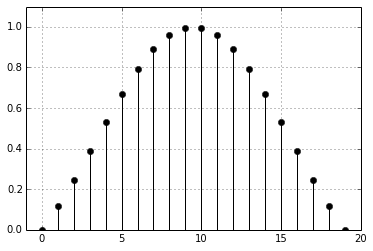
\includegraphics[width=1\columnwidth]{Figures/Example}
  \caption{Interactive data exploration with multiple devices.}
  \label{fig:example}
\end{figure}

$$\int{a,b}$$


\begin{figure}[h]
    \centering
    \subfigure[Figure A]{
    	\label{fig:a}
        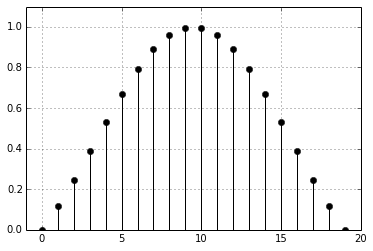
\includegraphics[width=60mm]{Figures/Example}
     }
	\subfigure[Figure B]{
    	\label{fig:b}
        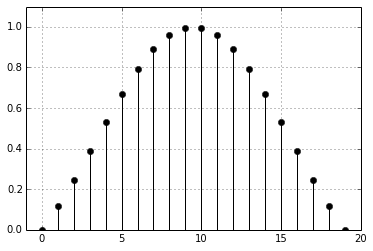
\includegraphics[width=60mm]{Figures/Example}
     }
    \caption{Wearables worn for experiments 1, 2, and 3.}\label{fig:figure2}
\end{figure}

Refer to a figure in the following forms:\\
If you take a look at Figure~\ref{fig:example} ...\\
... text text (see Figure~\ref{fig:example}) ...

\section{Listings}
\begin{lstlisting}[caption=A bit of source code., label=lst:test]
if( true == questions )
{
    std::cout << "Let me google it for you";
}
else
{
    std::cout << "Great";
}
\end{lstlisting}

Now lets take a look at Listing~\ref{lst:test}.


\section{Table}

\begin{table}[ht!]
  \caption{My caption with a very useful description. die kann auch etwas länger sein und über mehrere Zeilen gehen und so weiter.}
  \label{my-label}
  \begin{tabular}{llr}
    \hline
    \multicolumn{2}{c}{Item} &            \\ \cline{1-2}
    Animal     & Description & Price (\$) \\ \hline
    Gnat       & per gram    & 13.65      \\
               & each        & 0.01       \\
    Gnu        & stuffed     & 92.50      \\
    Emu        & stuffed     & 33.33      \\
    Armadillo  & frozen      & 8.99       \\ \hline
  \end{tabular}
\end{table}

For the fast generation of tables from Excel use \url{http://www.heise.de/download/excel2latex.html}

\section{Equations}

\LaTeX{} is great at typesetting equations. Let $X_1, X_2, \ldots, X_n$ be a sequence of independent and identically distributed random variables with $\text{E}[X_i] = \mu$ and $\text{Var}[X_i] = \sigma^2 < \infty$, and let

$$S_n = \frac{X_1 + X_2 + \cdots + X_n}{n}$$

This was a equation without a label.
      
\begin{equation}
S_n = \frac{1}{n}\sum_{i}^{n} X_i
\label{eq:test}
\end{equation}

This is the reference to equation~\ref{eq:test}.      

denote their mean. Then as $n$ approaches infinity, the random variables $\sqrt{n}(S_n - \mu)$ converge in distribution to a normal $\mathcal{N}(0, \sigma^2)$.




% /*================================
% =            CONTENTS            =
% ================================*/

\chapter{Preliminaries}
\label{ch:introduction}

Führt in die Thematik, Problem- und Aufgabenstellung ein

Vorstellung der Forschungsfrage

Enthält Grundlagenwissen

Gibt Überblick über die Arbeit

Darstellung der Related Work - sofern bereits ähnliche Arbeiten zu diesem Themengebiet existieren; In aller Kürze: Was gibt es? Was sind die Ergebnisse? Ist etwas offen geblieben? Fehlt etwas?

\chapter{Analytical Mechanics}
\label{ch:method}
\section{Lagrangian Mechanics}
\begin{tcolorbox}
    For
\end{tcolorbox}
field theory lagrangian
the EOM are obtained when we stationarize the the action i.e. equation the Frechet derivative to zero
\subsection{Constraints}
\subsection{Lagrange Multipliers}
\begin{center}
\begin{tabularx}{0.99\textwidth} { 
		| >{\raggedright\arraybackslash}X 
		| >{\centering\arraybackslash}X 
		| >{\raggedleft\arraybackslash}X | }
	\hline
\textbf{Characteristic of Intertial Frame} & \textbf{Property of Lagrangian} & \textbf{Conserved Quantity} \\
	\hline
	Time homogeneous & Not explicit function of time & Total energy \\
	\hline
	Time homogeneous   & Invariant to translation  & Linear momentum  \\
	\hline
	Space isotropic   & Invariant to rotation  & Angular momentum  \\
	\hline
\end{tabularx}
			\end{center}
\section{Hamilton's Mechanics}
Hamilton's equations are written as,
\begin{tcolorbox}
	\begin{equation}
\dot{q}_{i} = \frac{\partial H}{\partial p_{i}}
\end{equation}
\begin{equation}
-\dot{p}_{i} = \frac{\partial H}{\partial q_{i}}
\end{equation}
\end{tcolorbox}
	
	Where,
	$$H = T + V = \sum_{i = 1}^{n} p_{i}q_{i} - \mathcal{L}$$
	$$P = \frac{\partial \mathcal{L}}{\partial \dot{q}}$$
\subsection{Modified Hamilton's Principle}
We can thus modify Hamilton's principle to incorporate the Hamiltonian as,
\begin{equation}
\delta \int_{t_{1}}^{t_{2}} \left(\sum_{i = 1}^{n} p_{i}q_{i} - H \right) dt = 0 
\end{equation}
\subsection{Poisson Brackets}
We define Poisson Brackets as,
		\begin{equation}
		\{A, B\} = \sum_{i}^{n} \left( \frac{\partial A}{\partial q_{i}} \frac{\partial B}{\partial p_{i}} -  \frac{\partial B}{\partial q_{i}} \frac{\partial A}{\partial p_{i}}\right)
		\end{equation}
		They have the following properties,
		\begin{itemize}
		\item \textbf{Antisymmetry:} $\{A, C\} = -  \{C, A\}$
		\item \textbf{Bilinearity:} $\{kA, C\} = k \{A, C\}$
		\item $\{\left(AB\right), C\} = B\{A,C\} + A\{B,C\}$
		\end{itemize}
		
		We can rewrite Hamilton's equations through Poisson Brackets as,
		\begin{equation}
		\dot{p}_{i} = \{p_{i}, H\}
		\end{equation}
		\begin{equation}
		\dot{q}_{i} = \{q_{i}, H\}
		\end{equation}
		\begin{equation}
			\{q_{i}, p_{j}\} = \delta_{ij}
		\end{equation}
\section{Some Niche Stuff}
\subsection{Liouville's Theorem}
\subsection{Virial Theorem}
\begin{equation}
	S= \sum_{i}^{n} p_{i} . r_{i}
	\end{equation}
	\begin{equation}
	\frac{d S}{d t} = \sum_{i}^{n} \dot{p}_{i} . r_{i} + p_{i} . \dot{r}_{i}
	\end{equation}
	\begin{equation}
	\expectationvalue{\frac{d S}{d t}} = \frac{1}{\tau} \int_{0}^{r} \frac{d S}{d t} dt = \frac{S(\tau) - S(0)}{\tau}
	\end{equation}
	
	\begin{equation}
		\expectationvalue{\sum_{i}^{n} p_{i} . \dot{r}_{i}} = - \expectationvalue{\sum_{i}^{n} \dot{p}_{i} . r_{i}}
		\end{equation}
		\begin{equation}
		\expectationvalue{2 \sum_{i}^{n} T_{i}} = - \expectationvalue{\sum_{i}^{n} \dot{F}_{i} . r_{i}}
		\end{equation}
		\begin{equation}
		\expectationvalue{T} = - \frac{1}{2} \expectationvalue{\sum_{i}^{n} \dot{F}_{i} . r_{i}}
		\end{equation}
\section{Noether's Theorem}
\subsection{The Rund-Tutman Identity}

\chapter{Quantum Mechanics}
\label{ch:qm}

\section{State Vector}
\begin{itemize}
\item In Quantum Mechanics, we start with an object called the state vector $\ket{\psi}$. All the information about the system is contained in it. 
\item The position basis representation of the state vector is called the wavefunction $\psi (\vec{x}, t) = \braket{x}{\psi}$.
\item If we wish to know about a particular physical measurable such as an object's position of momentum, we can extract this information from the State vector by means of acting on with an Operator that corresponds to the measurable quantity.
\end{itemize}
\subsection{Admissibility Conditions for a Wavefunction}
A physically relevant wavefunction must be:
\begin{itemize}
\item Continuous i.e. no singularities in it's topology
\item Smooth i.e. a Taylor expansion for it exists
\item Quadratically integrable with the integral being single valued i.e. finite everywhere and $\psi \rightarrow 0$ as $r \rightarrow \infty$
\item Forming an orthonormal set
\item Satisfying the boundary conditions of the quantum mechanical system it represents
\end{itemize}
\section{Observables}
\begin{itemize}
\item Observable quantities such as position and momnetum c
\end{itemize}

\section{Time Evolution}
\subsection{Schrodinger Picture}
Where\\
If we consider the Schrodinger picture i.e. the state vector evovles with time whereas the Observables are in a loose sense eternal. The time evolution of the state vector is given by the Schrodinger equation:
\begin{equation}
	i \hbar \frac{\partial \ket{\psi}}{\partial t} = \hat{H} \ket{\psi}
\end{equation}
Or,
\begin{equation}
	i \hbar \frac{\partial \psi}{\partial t} = \hat{H} \psi
\end{equation}
in terms of the Wavefunction. Where, $\hat{H}$ is the Hamiltonian operator, which can be expressed as:
\begin{equation}
	\hat{H} = -\frac{\hbar^{2} \nabla^2}{2m} + V(\vec{x})
\end{equation}
for a free particle. 

\subsection{Heisenberg Picture}

\section{Measurement}
Measurement is defined as a form of time-evolution that is non-unitary and non-deterministic. 
According to Born's rule
\begin{equation}
	\int_{a}^{b} \abs{\psi(\vec{x}, t)}^{2} dx = \text{Probability of finding the particle at a time t between positions a and b}
\end{equation}
Thus, . Physically speaking this lends a kind of indeterminancy to the wavefunction. We can only speak of probabilities. Therefore, we can only , this brings to the measurement hypothesis, that is the State vector evolves to the state corresponding to the measurement being made. And unlike the Schrodinger equation, this evolution is non-deterministic. This tension is often called the "measurement problem", i.e. why is the measurement of an observable a special process distinct from others? Several theories and models claim to have resolved this, but we shall save that discussion for another time. We will fully focus on understanding the theory of Quantum Mechanics in a pragmatic lens before we question its foundations (although the converse isn't necessarily a bad thing, it isn't the purpose of this manuscript however).

\section{Summary of Postulates}
\begin{figure}
	\centering
	\includegraphics[scale=0.5]{delta-distribution.png}
	\caption{A Plot of $\delta(x)$}
\end{figure}
\section{Normalization}
Normalization is a process through which we ensure that,
\begin{equation}\label{norm}
	\int_{- \infty}^{\infty} \abs{\psi(\vec{x}, t)}^{2} dx = 1
\end{equation}
This is a natural consequence of Born's rule, we simply want all the probabilities to add up to 1. Thus, to rule out any other absurd scenarios, we make a ruling that non-Normalizable and non-square integrable Wavefunctions are unphysical.\\
We can also prove that once normalized, the wavefunction always remains normalized, we start by differentiating equation (\ref{norm}) with respect to time\\
$$\frac{d}{dt} \int_{- \infty}^{\infty} \abs{\psi(\vec{x}, t)}^{2} dx = \frac{\partial}{\partial t}\int_{- \infty}^{\infty} \abs{\psi(\vec{x}, t)}^{2} dx$$
Dealing with the term inside the integral,
$$ \frac{\partial}{\partial t}\abs{\psi(\vec{x}, t)}^{2} = \frac{\partial}{\partial t} (\psi^{*} \psi ) = \psi^{*}\frac{\partial \psi}{\partial t} + \psi\frac{\partial \psi^{*}}{\partial t}$$
Now the Schrodinger equation for a free particle reads as,
$$\frac{\partial \psi}{\partial t} = \frac{i \hbar}{2m}\frac{\partial^{2} \psi}{\partial x^{2}} - \frac{i}{\hbar}V \psi$$
Conjugating this we can see that,
$$\frac{\partial \psi^{*}}{\partial t} = -\frac{i \hbar}{2m}\frac{\partial^{2} \psi^{*}}{\partial x^{2}} + \frac{i}{\hbar}V \psi^{*}$$
Thus,
$$\frac{\partial}{\partial t}\abs{\psi(\vec{x}, t)}^{2} = \frac{i \hbar}{2m}\left( \psi^{*} \frac{\partial^{2} \psi}{\partial x^{2}} - \psi \frac{\partial^{2} \psi^{*}}{\partial x^{2}} \right) = \frac{\partial }{\partial x}\left[\frac{i \hbar}{2m}\left( \psi^{*} \frac{\partial \psi}{\partial x} - \psi \frac{\partial \psi^{*}}{\partial x} \right)\right]$$
Now we evaluate the integral,
$$\frac{d}{dt} \int_{- \infty}^{\infty} \abs{\psi(\vec{x}, t)}^{2} dx = \frac{i \hbar}{2m}\left( \psi^{*} \frac{\partial \psi}{\partial x} - \psi \frac{\partial \psi^{*}}{\partial x} \right)^{\infty}_{- \infty} $$
But $\psi$ must go to zero as goes to infinity, otherwise the wave function would not be normalizable. Thus it follows that.
\begin{equation}
	\frac{d}{dt} \int_{- \infty}^{\infty} \abs{\psi(\vec{x}, t)}^{2} dx = 0
\end{equation}
And hence, the integral is constant i.e. independent of time. Therefore if is normalized at a time $t = 0$, it remains normalized for all future. 
\section{Generalized Uncertainty Principle}
Suppose we have a ket $\ket{\psi}$ and two operators $\hat{A}$ and $\hat{B}$, we define two new vectors

$$,$$

$$,$$

We use the Cauchy-Shwarz inequality,

$$ 2|X||Y| \geq |\langle X|Y \rangle + \langle Y|X \rangle |$$

Substituting in the left-hand side,
$2\sqrt{\langle X|X\rangle\langle Y|Y\rangle} \geq |\langle X| Y  \rangle+ \langle Y | X \rangle|$
Plugging in Eqs. (4) and (5),
$2\sqrt{\langle \psi |A^{2} |\psi \rangle \langle \psi | -B^{2}| \psi \rangle} \geq |\langle X | Y \rangle + \langle Y | X \rangle |$
Taking the $-1$ outside,
$2i\sqrt{\langle \psi |A^{2} |\psi \rangle \langle \psi | B^{2}| \psi \rangle} \geq |\langle X | Y \rangle + \langle Y | X \rangle|$
We now substitute in the right hand of the equation
$2i\sqrt{\langle \psi |A^{2} |\psi \rangle \langle \psi | B^{2}| \psi \rangle} \geq | \langle {\psi} |\hat{A}\hat{B}| {\psi} \rangle - \langle {\psi} |\hat{B}\hat{A}| {\psi} \rangle|$
The negative sign is due to the $i$, this also seems to represent the commutator, so we substitute
$2i\sqrt{\langle \psi |A^{2} |\psi \rangle \langle \psi | B^{2}| \psi \rangle }\geq |\langle\psi |[\hat{A},\hat{B}]|\psi\rangle$
Again, the right hand side looks like the expectation value of a quantity, so
$2i\sqrt{\langle A^{2} \rangle \langle B^{2} \rangle} \geq |\langle [\hat{A},\hat{B}] \rangle |$
$\sqrt{\langle A^{2} \rangle \langle B^{2} \rangle} \geq \frac{1}{2i} |\langle [\hat{A},\hat{B}] \rangle |$
We use Eq. (2),

$\sqrt{\sigma_{A}^{2}\sigma_{B}^{2}} \geq \frac{1}{2i} |\langle [\hat{A},\hat{B}] \rangle|$
Removing the square root we get the expression:
$\sigma_{A}\sigma_{B} \geq \frac{1}{2i} |\langle[\hat{A}, \hat{B}]\rangle|$

This is called the generalized uncertainty principle. This basically states that two variables that do not commute cannot be measured with precision simultaneously.

Talking about position and momentum

We know that observable properties can be represented using operators, here we'll 

$\hat{x} = x$
$\hat{P} = -i\hbar \frac{\partial}{\partial x}$
So we now try to find the commutator now
$[\hat{x}, \hat{p}] = \hat{x}\hat{p} - \hat{p}\hat{x}$
$[\hat{x}, \hat{p}] = -ix\hbar \frac{\partial}{\partial x} + i\hbar \frac{\partial}{\partial x}$
Now let's apply this to state vector to obtain the expectation value
$[\hat{x}, \hat{p}] |\psi\rangle = -ix\hbar \frac{\partial}{\partial x} |\psi\rangle + i\hbar \frac{\partial x|\psi\rangle}{\partial x}$
$$[\hat{x}, \hat{p}] |\psi\rangle = -ix\hbar \frac{\partial}{\partial x} |\psi\rangle + ix\hbar \pdv{(|\psi\rangle)}{x} + i\hbar$$
$[\hat{x}, \hat{p}] |\psi\rangle = i\hbar$
Substituting this into Eq.(),
$\sigma_{x}\sigma_{p} \geq \frac{1}{2i} i\hbar$
$\sigma_{x}\sigma_{p} \geq \frac{\hbar}{2}$ 
$\sigma_{x}\sigma_{p} \geq \frac{h}{4 \pi}$
\section{Summary of Consequences}
\begin{figure}
	\centering
	\includegraphics[scale=0.5]{delta-distribution.png}
	\caption{A Plot of $\delta(x)$}
\end{figure}
\section{Generalized Statistical Interpretation}
. \footnote{There of course exist other interpretations with subtle variations, we will discuss about these in Chapter \ref{epi}} If you measure an observable $\hat{O}$ on a particle in the state $\psi()$, you will certainly get one of the eigenvalues of the observable. If the spetra is discrete, the probability of getting the particular eigenvalue $q_{n}$ associated with the orthonormalized eigenfunction $f_{n}(x)$ is
\begin{equation}
	P(q_{n}) = \abs{c_{n}}^{2} = \abs{\braket{f_{x}}{\psi}}^{2}
\end{equation}
\subsection{Position Measurements}

\subsection{Momentum Measurements}

\section{Stationary State}
A  stationary state $\psi_{0}$ is a quantum mechanical state:
\begin{itemize}
\item with all observables independent of time
\item an eigenvector of the Hamiltonian
\item corresponds to a state with a single definite energy
\end{itemize}
Stationary states themselves are not constant in time but their probability densities $\abs{\psi_{0}}^{2}$ are
\section{The Continuity Equation}
\begin{tcolorbox}
\begin{equation}
\frac{\partial \rho}{\partial t} = - \nabla . \vec{J}
\end{equation}
\end{tcolorbox}
Where,
$$\rho = \psi \psi^{*}$$
$$\vec{J} = \frac{\hbar}{2mi} \left[ \psi^{*} \nabla \psi - (\nabla \psi^{*})\psi\right]$$
represents an interesting conservation law for quantum mechanics. But first, let's try to quickly prove this. 
\subsection{Proof}
W.k.t,
$$\frac{\partial}{\partial t}\int_{- \infty}^{\infty} \abs{\psi(\vec{x}, t)}^{2} dv = \frac{\partial}{\partial t}\int_{- \infty}^{\infty} \psi \psi^{*} dv = \int_{- \infty}^{\infty}  \psi^{*} \frac{\partial \psi}{\partial t} dv + \int_{- \infty}^{\infty}  \psi \frac{\partial \psi^{*}}{\partial t} dv = 0$$
\subsection{Interpretation}
\begin{itemize}
\item Probability is conserved i.e. $\sum_{i}^{\infty}P_{i} = 1$ \footnote{This holds well in the non-relativistic case i.e. when there is no creation or annihilation of particles}
\item The probability density evolves deterministically
\end{itemize}
\section{The Density Matrix}

\subsection{Properties}
\begin{itemize}
\item $\rho^{\dagger} = \rho$
\item$\Tr \rho= 1$
\item For a pure ensemble:
\begin{itemize}
\item $\rho^{2} = \rho$
\item $\Tr \rho^{2} \leq 1$
\end{itemize}
\item For an ensemble uniformly distributed over $k$ states: $\rho = (1/k)\mathbb{I}$
\end{itemize}
\chapter{Multiple Particles}
\label{ch:discussion}

Comparison of presented technologies/methods/projects

Kritische Diskussion / Vergleich der Ansätze

Welche Methoden werden zumeist genutzt, warum?

Überblick / Zusammenfassung der gefundenen Literatur in einer sinnvollen Kategorisierung / Charakterisierung

\chapter{Field Theory}
\section{What is a field?}


\pagestyle{plain} 

% References
\newpage
%\printbibliography
%\addcontentsline{toc}{chapter}{Bibliography}
%\ifUseGermanVersion
%	\bibliographystyle{fhstp-apalike}
%\else
%    \bibliographystyle{apa-good}
%\fi

%\bibliography{Bibliography.bib}

% Figures
\newpage
\listoffigures
\addcontentsline{toc}{chapter}{List of Figures}
% Tables
\newpage
\listoftables
\addcontentsline{toc}{chapter}{List of Tables}
% Listings
\newpage
\lstlistoflistings
\addcontentsline{toc}{chapter}{List of Listings}
\newpage

% ============================================

\chapter*{Appendices}
\setcounter{section}{0}

\addcontentsline{toc}{chapter}{Appendices}
\renewcommand{\thesection}{\Alph{section}}

\section{Mathematical Preliminaries}
\label{appendix_a}
\subsection{Sets}
\subsubsection{The Axiom of Extension}
\subsubsection{The Axiom of Specification}
\subsubsection{Unordered Pairs}
\subsubsection{Unions and Intersections}
\subsubsection{Complements and Powers}
\subsubsection{Ordered Pairs}
\subsubsection{Relations}
\subsubsection{Maps}
\subsubsection{Families}
\subsubsection{Cartesian Product}
Here the symbol "$\times$" means \textbf{"Cartesian Product"} i.e. it's action w.r.t two sets $\mathbb{A}$ and $\mathbb{B}$ is the set of all ordered pairs $(a, b)$ where $a \in \mathbb{A}$ and $b \in \mathbb{B}$
\subsection{Logic}

\subsection{Complex Numbers}
\label{appendix_a}
A complex number is an ordered pair $z = \{a,b\} \in \mathbb{C}$ where $a,b \in \mathbb{R}$ where we can denote it as $z = a + ib$ where $i = \sqrt{-1}$
\subsubsection{Addition}
$z_{1} = a_{1} + ib_{1}, \ z_{2} = a_{2} + ib_{2}$
$$z_{1} + z_{2} =  (a_{1} + a_{2}) + i(b_{1} + b_{2})$$
\subsubsection{Multiplication}
$z_{1} = a_{1} + ib_{1}, \ z_{2} = a_{2} + ib_{2}$
$$z_{1}z_{2} =  (a_{1} + ib_{1})(a_{2} + ib_{2}) = (a_{1}a_{2} - b_{1}b_{2}) + i(a_{1}b_{2} + a_{2}b_{1})$$
\subsubsection{Properties}\footnote{$\mathcal{W}, \mathcal{Z}, \lambda \in \mathbb{C}$}
\subsubsubsubsection{Commutativity}
$$\mathcal{W} + \mathcal{Z} = \mathcal{Z} + \mathcal{W}$$
$$\mathcal{W}\mathcal{Z} = \mathcal{Z}\mathcal{W}$$
\subsubsubsubsection{Associativity}
$$(\mathcal{Z}_1 + \mathcal{Z}_2) + \mathcal{Z}_3 = \mathcal{Z}_1 + (\mathcal{Z}_2 + \mathcal{Z}_3)$$
$$(\mathcal{Z}_1\mathcal{Z}_2)\mathcal{Z}_3 = \mathcal{Z}_1(\mathcal{Z}_2\mathcal{Z}_3)$$
\subsubsection{Identities}
$$\mathcal{Z} + 0 = \mathcal{Z}$$
$$\mathcal{Z}1 = \mathcal{Z}$$
\subsubsubsubsection{Additive Inverse}
$$\forall \ \mathcal{Z} \ \exists \ \mathcal{Z}^{-1} \ | \ \mathcal{Z} + \mathcal{Z}^{-1} = 0$$
\subsubsubsubsection{Multiplicative Inverse}
$$\forall \  \mathcal{Z} \neq 0 \ \exists \ \mathcal{W} \ | \ \mathcal{Z}\mathcal{W} = 1$$
\subsubsubsubsection{Distributive Property}
$$\lambda(\mathcal{W} + \mathcal{Z}) = \lambda\mathcal{W} + \lambda\mathcal{Z}$$



\section{Fourier Analysis}
Fourier analysis is the study of a special set of an integral transforms. 
A fourier series is the decomposition of a general wave or oscillation into harmonic components.
Because we treat the wave vector as the independent variable of a wave, the Fourier decomposition
is typically done in terms of wave vectors. A Fourier series is a sum of sinusoidal functions, each of
which is a harmonic of some fundamental wave vector or spatial frequency. A Fourier transform is an
integral over a continuous distribution of sinusoidal functions.
A Fourier series is appropriate when the system has boundary conditions that limit the allowed
wave vectors to a discrete set. For a system where the spatial periodicity is $2L$, the Fourier decomposition of a general periodic function is the series
\begin{equation}
f(x) = \sum_{-\infty}^{\infty} c_{n}e^{i k_{n}x}
\end{equation}
where,
$$k_{n} = \frac{n \pi}{L}$$
Here $c_{n} \in \mathbb{C}$. All $f(x) \in \mathbb{R}$ can be written as:
\begin{equation}
f(x) = \frac{a_{0}}{2} + \sum^{\infty}_{n=1} \left[a_{n}\cos \left(\frac{n \pi x}{L} \right) + b_{n}\sin \left(\frac{n \pi x}{L}\right) \right]
\end{equation}
Where,
\begin{equation}
	a_{n} = \frac{1}{L} \int_{0}^{2L} f(x) \cos\left(\frac{n \pi x}{L}\right) dx
\end{equation}
\begin{equation}
	b_{n} = \frac{1}{L} \int_{0}^{2L} f(x) \sin\left(\frac{n \pi x}{L}\right) dx
\end{equation}
\begin{equation}
	c_{n} = \frac{1}{2L} \int_{0}^{2L} f(x) e^{-ik_{n}x}dx
\end{equation}
obtained by calculating the overlap integrals (i.e., projections or inner products) of the desired function with the harmonic basis functions. That is provided $f(x)$, obeys the following conditions i.e. \textbf{Dirichlet conditions}:
\begin{itemize}
\item It must be absolutely integrable over a period.
\item It must be of bounded variation in any given bounded interval.
\item It must have a finite number of discontinuities in any given bounded interval, and the discontinuities cannot be infinite.
\end{itemize}
A Fourier transform is appropriate when the system has no boundary conditions that limit the allowed wave vectors. In this case, the Fourier decomposition is an integral over a continuum of wave vectors:
\begin{equation}
	f(x) = \frac{1}{\sqrt{2 \pi}} \int_{-\infty}^{\infty} a(k)e^{ikx}dk
\end{equation}
where  the  expansion  function  $a(k)$  is  complex. To  obtain  the  expansion  function  $a(k)$  for  a  givenspatial function $f(x)$ requires the inverse Fourier transform
\begin{equation}
	a(k) = \frac{1}{\sqrt{2 \pi}} \int_{-\infty}^{\infty} f(x)e^{-ikx}dx
\end{equation}
which is a projection of the spatial function $f(x)$ onto the harmonic basis functions $e^{ikx}/\sqrt{2 \pi}$. The basis functions are orthogonal and normalized in the Dirac sense, which means their projections onto each other are Dirac delta functions
\begin{equation}
\begin{split}
	\frac{1}{2 \pi} & \int_{-\infty}^{\infty} e^{ik^{'}x}e^{-ikx}dx = \delta(k-k^{'})\\
	\frac{1}{2 \pi} & \int_{-\infty}^{\infty} e^{ikx^{'}}e^{-ikx}dk = \delta(x-x^{'})
\end{split}
\end{equation}
\subsection{Parseval’s theorem}
Parseval’s theorem states that the power is the same whether calculated in position space or wave-vector space:
\begin{equation}
\int^{\infty}_{-\infty} \abs{f(x)}^{2}dx = \int^{\infty}_{-\infty} \abs{a(k)}^{2}dk
\end{equation}

\section{The Dirac Delta Function}
\subsection{The Divergence of $\frac{\hat{r}}{r^{2}}$}
We can see why the divergence is,
\begin{equation}
\nabla . \frac{\hat{r}}{r^{2}} = 0
\end{equation}
But if we calculate this using the Divergence theorem, we find that ,
\begin{equation}
	\oint v .da = \int \left( \frac{\hat{r}}{r^{2}} \right) . \left( r^{2} \sin(\theta) d \theta d \phi \hat{r} \right) = \left( \int_{0}^{\pi} \sin(\theta) d \theta \right) \left( \int_{0}^{2\pi} d \phi \right) = 4 \pi
\end{equation}
This is paradoxical. The issue is that it blows up at $r=0$ but is is neglible everywhere else. How do we fix this? The Dirac Delta functional!
\subsection{The One-Dimensional Dirac Delta Functional}
The Dirac Delta is a functional \footnote{An object that is a map between functions} which we define as,
\begin{equation} \label{deltadef}
\delta(x-a)= 
\begin{cases}
0, & \text{if } x \neq a\\
\infty,              & \text{if } x = a
\end{cases}
\end{equation}
\begin{equation}
\int_{- \infty}^{+ \infty} \delta(x-a) dx = 1
\label{del2}
\end{equation}
$\forall \  a \in \mathbb{R}$
We can visualize it as a sharp peak at $a$,
\begin{figure}
	\centering
	\includegraphics[scale=0.5]{Figures/delta-distribution.png}
	\caption{A Plot of $\delta(x)$}
\end{figure}
We can interpret \ref{del2} as saying "the area of the delta distribution is always 1".
\begin{equation}
f(x)\delta(x - a ) = f(a)
\end{equation}
We can combine these to get,
\begin{equation}
\int_{- \infty}^{+ \infty} \delta(x-a) f(x) dx = f(a)
\end{equation}
\subsubsection{A few interesting properties}
\begin{equation}
\delta(kx) = \frac{1}{|k|}\delta(x)
\end{equation}
\begin{equation}
\frac{d}{dx}(\delta(x)) = -\delta(x)
\end{equation}
where k is a constant
\begin{equation}
\frac{d \theta}{dx} = \delta(x)
\end{equation}
Where $\theta$ is the step function defined as,
\begin{equation}
\theta(x)= 
\begin{cases}
1, & \text{if } x > 0\\
o,              & \text{if } x \leq 0
\end{cases}
\end{equation}

\subsection{The Three-Dimensional Dirac Delta Function}
We generalize (\ref{deltadef}) to three dimensions,
\begin{equation}
\delta^{3}(\vec{r} - \vec{a}) = \delta(x-a_{x})\delta(y-a_{y})\delta(z-a_{z})
\end{equation}
\begin{equation}
\int_{- \infty}^{+ \infty} \delta^{3}(\vec{r} - \vec{a}) dV = 1
\end{equation}
We can also define the three-dimensional delta function as
\begin{equation}
\delta^{3}(\boldscriptr) = \frac{1}{4 \pi} \left[\nabla \cdot \left( \frac{\hat{\boldscriptr}}{{\scriptr	}^{2}}\right)\right]
\end{equation}
Since,
$$\nabla \left(\frac{1}{\scriptr}\right) = -\frac{\hat{\boldscriptr}}{\scriptr^{2}}$$
We can rewrite as,
\begin{equation}
\delta^{3}(\boldscriptr) = -\frac{1}{4 \pi} \left[\nabla^{2}  \left( \frac{1}{\scriptr}\right)\right]
\end{equation}
\subsection{Integral representation}
We have the relationship for the Fourrier transform,
\begin{equation}
F(x) = \int f(t) e^{-ixt} dt
\end{equation}
and it's inverese
\begin{equation}
f(t) = \frac{1}{2 \pi} \int F(x) e^{ixt} dx
\end{equation}
Plugging in Eq. into Eq. we find that 
\begin{equation}
	F(y) = \frac{1}{2 \pi} \int_{-\infty}^{\infty} F(x) dx \int_{-\infty}^{\infty}e^{i(x-y)t} dt
\end{equation}	
Now, invoking the definig property of the Delta function,
\begin{equation}
F(y) = \int_{-\infty}^{\infty} F(x) \delta(x-y) dx
\end{equation}
Comparing and we find that,
\begin{tcolorbox}
\begin{equation}
\delta(x-y) = \frac{1}{2 \pi} \int_{-\infty}^{\infty} e^{i(x-y)t} dt
\end{equation}
\end{tcolorbox}

\section{Linear Algebra}
\label{appendix_a}
\subsection{Vector Spaces}
A linear vector space or simply a vector space $\mathbb{V}$ is a set along with the multiplication $(.)$ and addition $(+)$ operations over a field $\mathcal{F}$, such that the following axioms hold:
\begin{itemize}
	\item \textbf{Commutativity:} $\ket{u} + \ket{v} = \ket{v} + \ket{u}$
	\item \textbf{Associativity:} $(\ket{u} + \ket{v}) + \ket{w} = \ket{v} + (\ket{u} + \ket{w})$
	\item \textbf{Additive Identity:} 
	$\exists \  \ket{0} \in \mathbb{V} \ | \ \ket{v} + \ket{0} = \ket{0} + \ket{v} = \ket{v}$
	\item \textbf{Additive Inverse:} $\forall \ \ket{v} \ \exists \ \ket{v^{-1}} \ | \ \ket{v} + \ket{v^{-1}} = 0$
	\item \textbf{Multiplicative identity:} $\exists \ 1 \in \mathbb{V} \ | \ 1 .\ket{v} = \ket{v}$
	\item \textbf{Multiplicative Associativity:}  $(\alpha \beta) \ket{v} = \alpha (\beta \ket{v})$
	\item \textbf{Distributive Properties:} 
	\begin{itemize}
		\item $(\alpha + \beta) \ket{u} = \alpha \ket{u} + \beta \ket{u}$
		\item $\alpha (\ket{u} + \ket{v}) = \alpha \ket{u} + \alpha \ket{v}$
	\end{itemize}
\end{itemize}
Here, $\alpha , \beta \in \mathcal{F}$ and $\ket{u}, \ket{v} $ and $\ket{w} \in \mathbb{V}$
\subsection{Subspaces}
Given a vector space $\mathbb{V}$, a subset of its elements that form a vector space among themselves is called a subspace. We will denote a particular subspace $i$ of dimensionality $n_{i}$ by $\mathbb{V}^{n_{i}}_{i}$.\\
   Given two subspaces, and , we define their sum $\mathbb{V}^{n_{i}}_{i} \oplus \mathbb{V}^{m_{i}}_{i} = \mathbb{V}^{l_{i}}_{i}$ as the set containing:
\begin{enumerate}
\item All the elements of $\mathbb{V}^{n_{i}}_{i}$
\item All the elements of $\mathbb{V}^{m_{j}}_{j}$
\item And all possible linear combinations of the above
\end{enumerate} 
However for the elements of (3), closure is lost. The dimensionality of such a subspace is $n + m$.
\subsection{Bases, Span and Linear Independence}
\begin{itemize}
    \item If $S = \{\ket{v}_{1},\ket{v}_{1},...,\ket{v}_{k}\} \subset \mathbb{V}$ is a set of $k$ vectors in $\mathbb{V}$, then the span of $S$, denoted $Span \{\ket{v}_{1},\ket{v}_{2},...,\ket{v}_{k} \}$ or Span S, is defined to be just the set of all vectors of the form $\{c^{1}\ket{v}_{1} + c^{2}\ket{v}_{2} + .... + c^{k}\ket{v}_{k} \}$
    \item Such vectors are known as linear combinations of the $v_i$, so Span $S$ is just the set of all linear combinations of the vectors in $S$
    \item A basis for a vector space $\mathbb{V}$ is a linearly independent set $\mathcal{B} \subset \mathbb{V}$ whose span is all of $\mathbb{V}$
    \item The dimension of a vector space $\mathbb{V}$, denoted $dim \ \mathbb{V}$ , is the number of
elements of any finite basis
\item If no finite basis exists, then we say that $\mathbb{V}$ is infinite dimensional.
\item Components are simply the scalar coefficients with respect to a specific basis
\item Vectors exist independently of any chosen basis
\item Vectors transform (contravairant) in the opposite way (the inverse of the original transformation matrix) to which it's basis transforms (covariant)
\end{itemize}

\subsection{Linear Maps}
A linear map/transformation is simply transformation $\hat{L}$ that
		\begin{itemize}
				\item Adds inputs or outputs, $\hat{L}(\ket{v} + \ket{w}) = \hat{L}(\ket{v}) + \hat{L}(\ket{w})$
			\item Scale the inputs or outputs, $\hat{L}(\alpha \ket{v}) = \alpha \hat{L}(\ket{v})$
		\end{itemize}
		Here, $\alpha  \in \mathcal{F}$ and $\ket{v} $ and $\ket{w} \in \mathbb{V}$
\subsection{Hermitian Forms}
Every vector space $\mathbb{V}$ has a dual space $\mathbb{V}^{*}$
\begin{itemize}
\item $\forall \ \ket{v} \ \exists \ \bra{w} := \ket{v} \rightarrow \mathbb{R}$
\item Much like a vector space, one can assign the dual space a Basis set $e^{i}$
\item It is common to set the basis up in a way that $$e^{i}(e_{j}) = \delta^{i}_{j} = \begin{cases}            1, &         \text{if } i=j,\\
            0, &         \text{if } i\neq j.
    \end{cases}$$
\end{itemize}
A non-degenerate Hermitian form on a vector space $\mathbb{V}$ is a function
$\langle \cdot | \cdot \rangle$ which assigns to an ordered pair of vectors $\ket{v}, \ket{w} \in \mathbb{V}$ a scalar, denoted $\braket{v}{w}$,
having the following properties:
\begin{itemize}
    \item \textbf{Linearity for the vectors:} $\bra{U}(\alpha\ket{V}+\beta\ket{W}) = \bra{U}\alpha\ket{V} + \bra{U}\beta\ket{W} = \alpha\braket{U}{V} + \beta\braket{V}{W}$
    \item \textbf{Hermicity/Skew-symmetry:} $\braket{V}{W} = {(\braket{W}{V})}^{*}$
    \item \textbf{Non-degeneracy:} For each $\ket{v} \neq 0 \in \mathbb{V}$, there exists $w \in \mathbb{V}$ such that $\braket{v}{w} \neq 0$
    \item \textbf{Positive-Definiteness:} $\braket{V}{V} > 0$, for all $\ket{V} \neq \ket{0}$
\end{itemize}
\begin{itemize}
    \item There exists a symmetric bilinear function $g$ that maps Vectors to Duals i.e. $g : = \ket{v} \rightarrow \bra{v}$
    \item $\bra{v}$ is termed the metric dual
\end{itemize}

\subsection{Kernels}
For any linear map $\hat{T}$, a Kernel is a set of all vectors whose image is the zero vector. We often denote this space as $Ker(\hat{T})$.

%\subsection{Inner Product}
%A (sesquilinear i.e. half-linear) inner product is a generalization of the dot product that we are familiar with. It is defined as follows, the operation $\langle . | . \rangle$
%\begin{itemize}
 %   \item \textbf{Skew-symmetry:} $\langle V | W \rangle = { \langle W | V \rangle}^{*}$
  %  \item \textbf{Positive semidefiniteness:} $\langle V | V \rangle \geq 0$,* unless and until *$| V \rangle = | 0 \rangle$
   % \item \textbf{Linearity for the vectors:} $\langle U | (\alpha | V \rangle+\beta | W \rangle) = \langle U | \alpha | V \rangle + \langle U | \beta | W \rangle = \alpha \langle U |  V \rangle+ \beta \langle V |  W \rangle$*
%\end{itemize}
%Where, $\alpha \in \mathbb{C}$ and $| U \rangle,| V \rangle,| W \rangle \in \mathbb{V}$ and $\langle U| ,\langle V |, \langle W| \in \mathbb{V}^{*}$

\subsection{Hilbert Spaces}
A Hilbert space is an inner product vector space $\mathcal{H}$ that
\begin{itemize}
    \item has an norm i.e. length defined as $||V|| =  \sqrt{\langle V | V\rangle}$
    \item  is complete i.e. all of it's Cauchy sequences converge
\end{itemize}
A Cauchy sequence is simply a sequence of numbers whose succeeding term is smaller than the preceding one and when taken to a limit it converges. That is if you have a sequence One can visualize this as the plot of a dampened oscillator.

\subsection{Tensors}
A tensor is defined as a multilinear i.e. linear in every argument map $T(r,s)$ of the form
\begin{equation}
    \underbrace{V \times V \times V \times ...}_\text{your comment} \times \underbrace{V^{*} \time V^{*} \time V^{*} \times ...}_\text{s-times} \rightarrow \mathbb{R}
\end{equation}
\subsection{The Tensor Product}
A tensor product operation of two vectors $V \otimes W$ is defined as a bilinear function that maps $V^{*} \times W^{*}$ to the underlying field whose action is defined as
\begin{equation}
    (v \otimes w)(h,g) = v(h)w(g) \ \forall \ h \in V^{*}, g \in W^{*}
\end{equation}
Often times, a tensor is simply the set of all coefficients put in a matrix for such a map.
\subsection{A few interesting tensors}
\subsubsection{Kronecker delta}
It simply has the ‘function’ of ‘renaming’ an index:
$$\delta^{\mu}_{\nu} x^{\nu} = x^{\mu}$$
it is in a sense simply the identity matrix.
\subsubsection{Levi-Civita Pseudotensor}
\label{Levi}
The Levi-Civita Pseudotensor i.e. Tensor density is a completely anti-symmetric i.e. $\epsilon_{ijk} = -\epsilon_{jik} = -\epsilon_{ikj} = -\epsilon_{kji}$, we define it as:
\begin{equation}
\epsilon_{ijk} = \begin{cases}
1 \ \text{if } ijk \text{ is an even permuation of } 123\\
-1 \ \text{if } ijk \text{ is an odd permuation of } 123\\
0  \text{ if two indices are equal}\\
\end{cases}
\end{equation}
We have the identity
\begin{equation}
\epsilon_{\alpha \beta \nu}\epsilon_{\alpha \beta \sigma} = \delta_{\mu \rho} \delta_{\nu \sigma} - \delta_{\mu \sigma}\delta_{\nu \rho}
\end{equation}
From this it follows that,
\begin{equation}
\epsilon_{\alpha \beta \nu}\epsilon_{\alpha \beta \sigma} = 2\delta_{\nu \sigma}
\end{equation}
and
\begin{equation}
\epsilon_{\alpha \beta \gamma}\epsilon_{\alpha \beta \gamma} = 6
\end{equation}
Using these identities and the definition we can rewrite the cross-product of two vectors as,
\begin{equation}
\vec{a} = \vec{a} \cross \vec{b}  = \epsilon_{ijk}a_{j}b_{k}
\end{equation}
Thus the expressions in vector product notation can be changed to index notation for example,
$$
c = \nabla.(\nabla \cross \vec{a}) = \nabla_{i}(\epsilon_{ijk}\nabla_{j}a_{k}) = \epsilon_{ijk}\partial_{i}\partial_{j}a_{k}
$$
because,
$$\nabla_{i} = \frac{\partial}{\partial x_{i}} := \partial_{i}$$

\section{Complex Analysis}
\label{appendix_c}
\subsection{Analytic Functions}
A complex valued function, 
\begin{equation}
    f(z) = u(x,y) + iv(x,y)
\end{equation}
for $z = x + iy$ is said to be analytic in a region close to a point $z$, then it has a derivative at every point in that region i.e. neighbourhood. We define it's derivative as:
\begin{equation}
   f^{'}(z)  = \frac{df}{dz} = \lim_{\delta z  \rightarrow 0}\frac{\delta f(z + \delta z) - f(z)}{\delta z}
\end{equation}
An important point here is that $f^{'}(z)$ should not depend on the way $\delta z$ is selected. An alternate way to state this is to mandate that the Cauchy-Riemann relations,
\begin{equation}
    \begin{aligned}
    \frac{\partial u}{\partial x} = \frac{\partial v}{\partial y} \\
    \frac{\partial v}{\partial x} = - \frac{\partial u}{\partial y}
    \end{aligned}
\end{equation}
hold for $f(z)$.
\subsection{Poles}
A pole is a type of singularity i.e. a point where a mathematical object is not defined
. Think of the function $1/ z^{n}$ at $z = 0$. Let's suppose a function $f(z)$ is analytic between $C_{1}$ and $C_{2}$. In the region between them we can expand out $f(z)$ about a point $z_{0}$ as a Laurent series
\begin{equation}
    f(z) = a_{0} + a_{1} {(z- z_{0})} + a_{2} {(z- z_{0})}^{2} + ... + \frac{b_{1}}{{(z- z_{0})}} + \frac{b_{1}}{{(z- z_{0})}^{2}} + ...
\end{equation}
The part of the series with the b coefficients is termed as the principal part of the series. From this we can draw a few conclusions:
\begin{itemize}
    \item If all $b_{i}$'s are zero then $f(z_{0})$ is analytical at $z = z_{0}$
    \item If all $b_{i}$'s after $b_{n}$ are zero then we can say 
\end{itemize}
\subsection{Contour Integrals}
A contour $C$ is a closed path in $\mathbb{C}$ with a finite number of corners that doesn't cross itself. We will now review interesting things about integrals around such contours as, often we want to do difficult integrals over real variables. These may
be turned into easier integrals if we form a contour in the complex plane
which includes the original domain of integration which turn out to be much more tractable. The art is in choosing the best contour to do the integral
\subsubsection{Cauchy's Theorem}
If $f(z)$ is analytic on and inside $C$, then
\begin{equation}
    \oint_{C} dz \ f(z) = 0
\end{equation}
\subsubsection{Cauchy's Integral Formula}
If $f(z)$ is analytic on and inside a simple closed curve $C$ and a point a inside the curve, then 
\begin{equation}
    f(a) = \frac{1}{2 \pi i} \oint_{C} dz \frac{f(z)}{z-a}
\end{equation}
\subsubsection{Residue Theorem}
If $f(z)$ has singularities at points $z_{i}$, then for a contour $C$ that encloses them we have
\begin{equation}
    \oint_{C}dz \ f(z) = 2 \pi i \sum_{i} \text{Residue} \ \text{at} \ f(z_{i}) \ \text{inside} \ C
\end{equation}
wherein the integral is evaluated anti-clockwise i.e. we do it clockwise and simply invert the sign
\subsection{Branch Cuts}

\subsection{Cauchy's Principal Value Method}

\section{Group Theory}
\label{appendix_d}
\subsection{Preliminaries}
\subsubsection{Definition of a Group}
Examples of groups: 
\subsubsection{Subgroup}
For a group $G(G, *)$, a subgroup $H \subseteq G$ is defined as a group with the same composition binary operator. The notation $H \leq G$ is often used to indicate that $H$ is a subgroup of $G$
\subsubsection{Multiplication Tables}
From this itself we can tell if a group is abelian, as an abelian group would have 
\subsubsection{Morphisms}
A \textbf{group homomorphism} $\phi : G \rightarrow H$ is a map between two groups $G(G, *)$ and $H(H, +)$ that preserves the group structure i.e.
\begin{equation}
    \phi(a * b) = \phi(a) + \phi(b) \ \forall \  a,b \in G
\end{equation}
This preserves the group structure because:
\begin{itemize}
    \item This maps identity elements to identity elements i.e. $\phi(e_G) = e_{H}$
    \item 
\end{itemize}
The \textbf{Kernel} of a group homorphism $\phi : G \rightarrow H$ is the set of all elements of $G$ that are sent to the identity of $H$ i.e. $ker\phi = \{ g \in G | \phi(g) = e_{G}\}$
\begin{tcolorbox}
\textbf{Proposition:} A group homomorphism $\phi: G \rightarrow H$ is injective if and only if it's Kernel is trivial i.e. $ker\phi = \{ e_{G} \}$
\end{tcolorbox}
Two groups $G$ and $H$ are said to be isomorphic i.e. $G \iso H$ if there exists an invertible group homomorphism $\phi : G \rightarrow H$ i.e. an isomorphism

\subsubsection{Cosets}
\subsection{Important Theorems}
\subsubsection{Lagrange's Theorem}
\begin{tcolorbox}
    For any finite group G, the order (number of elements) of every subgroup of G is  equal to the number of of left cosets of $H$ in $G$
\end{tcolorbox}
\subsubsection{Cayleys's Theorem}
\begin{tcolorbox}
    Every group $G$ is isomorphic to a subgroup of the symmetric group acting on $G$
\end{tcolorbox}

\subsection{Lie Groups}

\subsection{Representation Theory}

\subsection{Reducibility and Irreducibility}

\section{Variational Calculus}
\subsection{A Lemma}
If,
\begin{equation}
    \int_{a}^{b}A(t)\eta(t)dt =0
\end{equation}
where,
\begin{itemize}
    \item $\eta(a) = \eta(b) = 0$
    \item $A(t)$ and $\eta(t)$ are both twice differentiable in the closed interval $[a,b]$ 
\end{itemize}
then,
\begin{tcolorbox}
$A(t) = 0$ throughout $[a,b]$
\end{tcolorbox}
\subsubsection{Proof by Contradiction}
Suppose that there exists $A(c) \neq 0$ for some $a < c < b$. For definiteness let's also suppose that $A(c) > 0$. Due to the continuity of $A(t)$, an interval $[t_{1},t_{2}]$ about c but within $[a,b]$ exists on which A(t) > 0. However under these conditions we can construct a $\eta(t)$ that leads to the integral being non-zero. For example,
\begin{equation} \label{deltadef}
\eta(t) =  
\begin{cases}
{(t-t_{1})}^{3}{(t_{2}-t)}^{3}, & \text{for } t_{1} < t < t_{2}\\
0, & \text{for } t < t_{1} \text{ and } t > t_{2}
\end{cases}
\end{equation}
\subsection{Deriving the Euler-Lagrange Equations}
The goal here is to find the extremal of the functional
\begin{equation}
			J(\alpha) = \int_{x_{2}}^{x_{1}}f\{y(\alpha , x),y^{'}(\alpha , x);x \} dx
		\end{equation}
		That is $\forall \ \eta(x)$, we want to find
		\begin{equation}
		\left. \frac{\partial J}{\partial \alpha} \right |_{\alpha = 0}  = 0
		\end{equation}
		Where $\alpha$ is a parameter.We thus start by, parameterizing $y$ as,
		\begin{equation} \label{increment}
		    y(x) = y(0) + \alpha \eta(x)
		\end{equation}
	We can now take the derivative
\begin{equation}
\frac{\partial J}{\partial \alpha} = \frac{\partial}{\partial \alpha}\int_{x_{2}}^{x_{1}}f\{y(\alpha , x),y^{'}(\alpha , x);x \} dx
\end{equation}
$$\frac{\partial J}{\partial \alpha} = \int_{x_{2}}^{x_{1}} \left(\frac{\partial f}{\partial y}\frac{\partial y}{\partial \alpha} + \frac{\partial f}{\partial y^{'}}\frac{\partial y^{'}}{\partial \alpha} \right) dx$$
From Equation (\ref{increment}) we have
\begin{align}
\frac{\partial y}{\partial \alpha} = \eta(x) \ ; \  & \frac{\partial y^{'}}{\partial \alpha} = \frac{d \eta}{d x}
\end{align}
a
	$$\frac{\partial J}{\partial \alpha} = \int_{x_{2}}^{x_{1}} \left(\frac{\partial f}{\partial y}\eta(x) + \frac{\partial f}{\partial y^{'}}\frac{\partial \eta}{\partial x} \right) dx$$	
	\begin{itemize}
		\item The second term in the integrand can be integrated by parts:
	\end{itemize}
	$$\int_{x_{1}}^{x_{2}} \frac{\partial f}{\partial y^{'}}\frac{d \eta}{dx} dx = \left \frac{\partial f}{\partial y^{'}} \eta(x) \right |^{x_{2}}_{x_{1}} -\int_{x_{1}}^{x_{2}} \frac{d}{dx} \left(\frac{\partial f}{\partial y^{'}}\right)\eta(x) dx $$
	$$\frac{\partial J}{\partial \alpha} = \int_{x_{1}}^{x_{2}} \left(\frac{\partial f}{\partial y} - \frac{d}{dx}\frac{\partial f}{\partial y^{'}} \right) \eta(x) dx$$
	\begin{tcolorbox}
		\begin{equation}
		\frac{\partial f}{\partial y} - \frac{d}{dx}\frac{\partial f}{\partial y^{'}} = 0
		\end{equation}
	\end{tcolorbox}
\subsection{Special Notation}
	We have the equation
\begin{equation}
\frac{\partial J}{\partial \alpha} d\alpha = \int_{x_{1}}^{x_{2}} \left(\frac{\partial f}{\partial y} - \frac{d}{dx}\frac{\partial f}{\partial y^{'}} \right) \frac{\partial y}{\partial \alpha} d \alpha dx = 0
\end{equation}
It can be written as 
\begin{equation}
\delta J = \int_{x_{1}}^{x_{2}} \left(\frac{\partial f}{\partial y} - \frac{d}{dx}\frac{\partial f}{\partial y^{'}} \right) \delta y \ dx = 0
\end{equation}
where
\begin{equation}
\begin{cases}
\frac{\partial J}{\partial \alpha} d\alpha = \delta J\\
\frac{\partial y}{\partial \alpha} d\alpha = \delta y
\end{cases}
\end{equation}
The condition of extremum then becomes,
\begin{equation}
\delta J = \delta \int_{x_{1}}^{x_{2}} f\{y, y^{'}; x\} dx = 0
\end{equation}
Sometimes we term this the functional derivative i.e. the Frechet derivative
\begin{equation}
    
\end{equation}
\subsection{Constraints}
\subsection{Lagrange Multipliers} 
\subsection{Variational Calculus in Physics}
\subsection{The Legendre Transform}
The Legendre transform
\subsection{The Rund-Tutman Identity}

\section{Probability Theory}
\subsection{Basics}
Probability is a number between 1 and 0 assigned to a proposition i.e. the probability of a proposition $A$
\begin{equation}
    prob(A) \in [0,1]
\end{equation}

\subsection{Discrete Distributions}
Suppose we have a frequency distribution 
\begin{equation}
N = \sum_{j=0}^{\infty} N(j)
\end{equation}
The probability of an event $N_{j}$ is defined as,
\begin{equation}
P(j) = \frac{N(j)}{N}
\end{equation}
In probability theory, the sum of all probabilities is 1,
\begin{equation}
\sum_{j = 0}^{\infty}P(j) = \sum_{j = 0}^{\infty}\frac{N(j)}{N} = 1
\end{equation}
The average/mean/expectation value of a value $j$ is given by the formula:
\begin{equation}
	\expval{j} = \frac{\sum j N(j)}{N} = \sum_{j =0 }^{\infty} j P(j)
\end{equation}
and in general, the average of some function of $j$, is given by,
\begin{equation}
\expval{f(j)} = \sum_{j =0 }^{\infty} f(j) P(j)
\end{equation}
The spread of a variable's value from it's mean is called it's variance, written as
\begin{equation}
\sigma^{2} = \expval{{(\Delta j)}^{2}}
\end{equation}
where,
$$\Delta j = j - \expval{j}$$
It's square root is called the standard deviation,
\begin{equation}
\sigma = \sqrt{\expval{{(\Delta j)}^{2}}} =  \sqrt{\expval{j^{2}} - \expval{j}^{2}}
\end{equation}
Which comes from a theorem on variances that we'll find useful later on:
$$\sigma^{2} = \expval{{(\Delta j)}^{2}} = \sum {(\Delta j)}^{2} P(j) = \sum {(j- \expval{j})}^{2} P(j)$$
$$ = \sum (j^{2} - 2j \expval{j} + \expval{j}^{2}) P(j)$$
$$ = \sum j^{2}P(j) - 2 \expval{j} \sum jP(j) + \expval{j}^{2}\sum P(j)$$
$$ = \expval{j^{2}} - 2 \expval{j}\expval{j} + \expval{j}^{2} = \expval{j^{2}} - \expval{j}^{2}$$
\subsection{Continuous Distributions}
We now move to a continuous probability distribution, we'll create continuous analogs of all the quantities we just introduced. Let's start with probability, the probability of that $x$ lies between $a$ and $b$
\begin{equation}
	P_{ab} = \int_{a}^{b} \rho(x) dx
\end{equation}
where $\rho(x)$ is the called the probability density i.e. the probability of getting $x$, or more concretely,
$$\rho(x)dx = \text{Probability that an individual is chosend at random lies between } x \text{ and } x + dx$$
Now supposing the rules we held for discrete variables hold, the continuous analogs look like this:
\begin{equation}
	1 = \int_{- \infty}^{\infty} \rho(x) dx
\end{equation}
\begin{equation}
	\expval{x} = \int_{- \infty}^{\infty} x \rho(x) dx
\end{equation}
\begin{equation}
	\expval{f(x)} = \int_{- \infty}^{\infty} f(x) \rho(x) dx
\end{equation}
\begin{equation}
	\sigma^{2} := \expval{(\Delta x)^{2}} = \expval{x^{2}} - {\expval{x}}^{2}
\end{equation}
%\section{Expectation Values}
%In this section we'll explore how we express the expectation values of a few opeartors. Let's start with the position opeartor in the position representation (i.e. position basis):
%\begin{equation} \label{posex}
	%\expval{x} = \int_{- \infty}^{\infty} x \abs{\psi(\vec{x}, t)}^{2} dx
%\end{equation}
%We can differentiate \ref{posex} with respect to time to find the expectation value for "velocity":
%$$\frac{d \expval{x}}{dt} = $$
%Throwing away 
%\begin{equation}
%	\expval{v} = \frac{d \expval{x}}{dt} = -\frac{i \hbar}{m} \int \psi^{*} \frac{\partial \psi}{\partial x} dx
%\end{equation}
%Therefore we can write the expectation value of momentum as,
%\begin{equation}
%	\expval{p} = m \frac{d \expval{x}}{dt} =  -i \hbar \int \left(\psi^{*} \frac{\partial \psi}{\partial x} \right) dx
%\end{equation}
%In general, every observable is a function of position and momentum, thus for an observable %$\hat{O}(x,p)$, the expectation value is given by,
%\begin{equation}
%	\expval{\hat{O}(x,p)} = \int \psi^{*} \hat{O}(x,-i \hbar \nabla) \psi dx
%\end{equation}
%For example, the expectation value of kinetic energy is,
%\begin{equation}
%\expval{T} = -\frac{\hbar^{2}}{2m} \int \psi^{*} \frac{\partial^{2} \psi}{\partial x^{2}} dx
%\end{equation}
%Or to sum it up in Dirac notation,
%\begin{equation}
%	\expval{\hat{O}} = \expval{\hat{O}}{\psi}
%\end{equation}

%\printbibliography
\begin{thebibliography}{9}
	
	\bibitem{p} Baez, J. C., &amp; Muniain, J. P. (2011). Gauge fields, knots and gravity. Singapore: World Scientific.
	
	\bibitem{p} Griffiths, D. J. (2018). Introduction to electrodynamics. Cambridge, United Kingdom: Cambridge University Press.
	
	\bibitem {p} Lancaster, T., \& Blundell, S. (2018). Quantum field theory for the gifted amateur. Oxford: Oxford University Press.
	
	\bibitem {p} Neuenschwander, D. E. (2017). Emmy Noether's wonderful theorem. Baltimore: Johns Hopkins Univ. Press.
	
	 \bibitem {p} Aivazis, M., \& Tung, W. (2006). Group theory in physics. Singapore: World Scientific.
	
	\bibitem {p6} Schwichtenberg, J. (2018). Physics from Symmetry. Cham: Springer International Publishing.
	
	

\end{thebibliography}
% ============================================

\end{document}























